\chapter{Evidence of pentaquark states in $\Lb\to\jpsi\proton\pim$ decay}
\label{chap:pentaquark_jpsippi}


\section{Study motivation}
%\lhcb reported significant $\jpsi K$ mass structures in $\Lb\to\jpsi\proton\Km$ decays using Run 1 data sample,
%and the reflection from $\Lz^{*}\to\jpsi\Km$ contributions have been be excluded from full amplitude analysis\supercite{LHCb-PAPER-2015-029}.
%Then, cross check was performed in a nearly model independent way in Ref.~[\cite{LHCb-PAPER-2016-009}], 
%where it was shown that the $\jpsi\proton$ structure near 4450\mev was too narrow to be accounted for by a collection of $\proton\kaon$ contributions.
%more details are presented in Appendix.~\ref{app:pentaquark_study}.
%This reinforced the results from the earlier model dependent amplitude analysis of the same data\supercite{LHCb-PAPER-2015-029}, 
%in which the $P_{c}(4450)^{+}$ structure was determined to peak at $4449.8\pm 1.7\pm 2.5$ \mev, 
%have a width of $39\pm 5\pm 19$ \mev. 
%Even though not apparent from the $m(\jpsi\proton)$ distribution, 
%the amplitude analysis required also a second, 
%broad $\jpsi\proton$ state for a reasonable description of the data, 
%peaking at $4380\pm 8\pm 29$ \mev, 
%with a width of $205\pm18\pm86$\mev. 
%The spins of these structures were not determined, 
%though the data preferred spin combinations involving $3/2$ and $5/2$ in either order. 
%The spin-parity preferences exhibited significant $\Lz^{*}$ model dependence. 
%Investigation of the Argand diagrams for the $P_{c}(4450)^{+}$ and $P_{c}(4380)^{+}$ structures was inconclusive 
%because of the large statistical errors.


The Cabibbo-suppressed decay $\LbJpsippi$ offers a new possibility to study these two states, 
as well as the other type of exotic state $\ZC^-\to \jpsi \pim$. 
The study of the relative branching fraction $\RpiK\equiv\BF(\Lb\to\pim P_c^+)/\BF(\Lb\to \Km P_c^+)$ 
could be useful to discriminate among their possible interpretations.  
Starting from $\Lb$, $ud(b)$, 
the Cabibbo-suppressed  $\bquark\to\ccbar\dquark$ transition combined with the creation of a light quark pair $\uubar$ yields a final state 
with the quark content $ud(\ccbar d)u\uquarkbar$. 
The $\dquark$ quark in the $\Pcplus$ state can be either directly from the content in the $\Lb$ baryon or from the $b\to\ccbar\dquark$ transition. 
This results in two interfering processes, 
referred as the external $W$-emission and the internal $W$-emission diagrams~\supercite{Cheng:2015cca}.  
The two diagrams are shown in Figure.~\ref{fig:fenyman}. 
While for the Cabibbo-favoured decay $\Lb\to\Km\Pcplus$, 
only the external $W$-emission process exists, 
as the transition $b\to\ccbar\squark$ doesn't produce a $\dquark$ quark for the $P_c^+$ state. e
Assuming the internal $W$-emission process is zero, 
Ref.~[\cite{Cheng:2015cca}] predicted the relative branching fraction $\RpiK=0.07\sim 0.08$, 
due to the differences of CKM elements and the phase-space factors. 
A sizable internal $W$-emission process could modify (either increase or reduce) the predicted value and even the relative production phase 
between the two $P_c$ states, resulting in different interference patterns between the two decays.   

A different production mechanics is proposed. Ref.~[\cite{Hsiao:2015nna}] argues 
that the $\ZP$ state in the $\LbJpsipK$ decay is produced mainly by the charmless $\Lb$ decay via the $b\to\uubar\squark$ transition, 
in which the $\ccbar$ contents in $\ZP$ states arise from the intrinsic charms within the $\Lb$ baryon. 
The Feynman diagram is shown in Figure.~\ref{feyHsiao}. 
A very large value $\RpiK=0.58\pm0.05$ is predicted. 


\begin{figure}[!hbp]
\centering
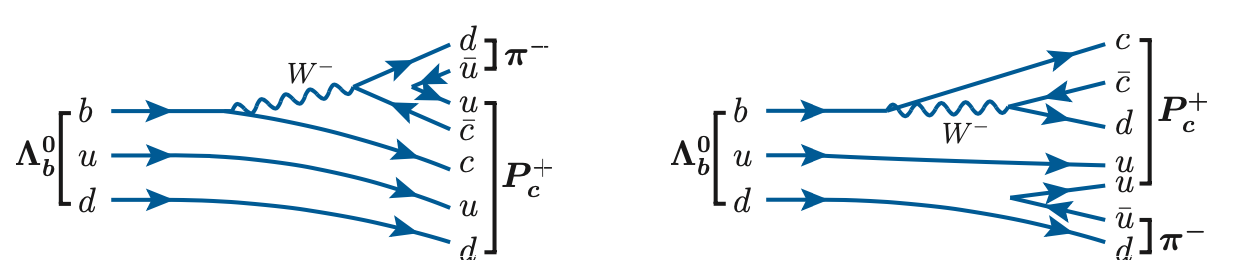
\includegraphics[trim=0 20  0 0, width=0.95\textwidth, clip=true]{Figures/04_Penta/01_introduction/Fenyman.png}
\caption{Feynman diagrams of the $\Lb\to\ZP\pi$ decay via (left) the external and (right) the internal $W^-$ emissions.}
\label{fig:fenyman}
\end{figure}



\begin{figure}[!tbp]
\centering
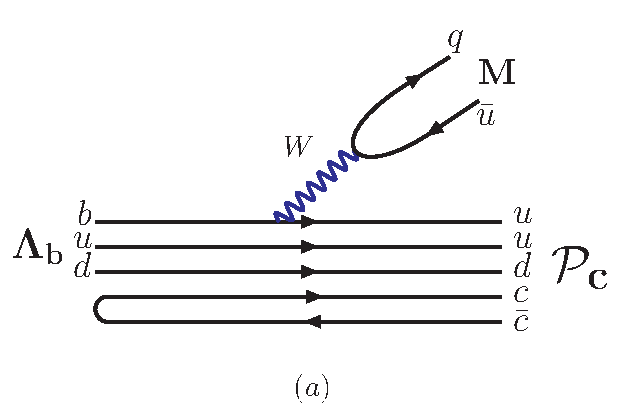
\includegraphics[trim=0 20  0 0, width=0.5\textwidth, clip=true]{Figures/04_Penta/01_introduction/intrinsic}
   \caption{Feynman diagram of $\Lb\to\Pcplus M$ via the charmless $b\to\uubar q$ transition suggested by Ref.~[\cite{Hsiao:2015nna}], 
   where $M(q)$ can be $\Km(s)$ or $\pim(d)$.}
   \label{feyHsiao}
\end{figure}


The channel $\LbJpsippi$ is expected to be produced via the intermedia resonances $\Nstar$, $\Lb\to\jpsi N^{*}$ with $N^{*}\to\proton\pim$.
The transition of $\Lb\to\jpsi N^{*}$ is dominated by the flavor changing decay of $b \to c+ \bar{c}d$. 
This suggests that the $\uquark$ and $\dquark$ quark in the $\Lb$ should be a spectator, 
hence their isospin quantum number $I = 0$ should be conserved. 
As a consequence, if the $ud$ pair is to be combined with a $d$ quark to form a baryon, 
it will favor $N$ baryons instead of $\Delta$ ones.

LHCb has measured the branching fraction of the overall Cabibbo-suppressed decay relative to the Cabibbo-favoured decay 
to be $\BF(\LbJpsippi)/\BF(\LbJpsipK)=0.0824\pm0.0024\pm0.0042$\supercite{LHCb-PAPER-2014-020}, 
where the first uncertainty is statistical and the second systematic.


Actually,
a full amplitude analysis of $\Lb\to\jpsi\proton\pim$ decay has been performed using \lhcb Run 1 data sample\supercite{LHCb-PAPER-2016-015}.  
If including both types of the exotic resonances report in 2015\supercite{LHCb-PAPER-2015-029},
the total significance for them is $3.1\sigma$ using a conservative model of $N^{*}$ resonances 
and $6.6\sigma$ when only well established $N^{*}$ states are allowed. 
Within the large statistical and systematic errors, 
the data are consistent with the $P_c{4450}^{+}$ and $P_c(4380)^{+}$ production rates expected from their previous observation and Cabibbo suppression.
However,
a new narrow $P_c(4312)^{+}$ state is discorved with a large statistical with Run 1 and Run 2 sample collected at \lhcb\supercite{LHCb-PAPER-2019-014}, 
and the previously reported $P_c(4450)^{+}$ structure contains two peaks,
$P_c(4440)^{+}$ and $P_c(4457)^{+}$,
which match the predictions for loosely bound and narrow molecular states.
In this case,
it is required to revisit this decay channel with both Run 1 and Run 2 data sample.




